\documentclass{article}
\usepackage[utf8]{inputenc}
\usepackage{amsmath, amssymb}
\usepackage{mathtools}
\usepackage{a4wide}
\usepackage{appendix}
\usepackage{listings}
\usepackage{float}
\usepackage{subcaption}
\usepackage{hyperref}
\usepackage{float}

\title{Salami}
\author{Hugo M. Nielsen (s214734) \and Mikael H. Hoffmann (s214753) \and Christian Valentin Kjær (s211469) \and Jacob Tuxen (s194572)}
\date{\today}

\begin{document}
\maketitle
\section{Problem and background}
When producing sausages and salami, determining the meat/fat ratio is of great interest. Manually annotating sausages and salami requires a food expert and this is very time and resource-consuming. 
Therefore we will look at this problem using image analysis and investigate whether it is possible to create a model that can automatically calculate the meat/fat ratio. The aim of this project is to create a model that is fit for fat and meat detection of sausages and find the most suitable ripeness state of sausage to perform our analysis - our analysis will be based on images of sausages.

To do this we assume that each pixel is an independent multivariate normal distribution and can therefore be classified into either meat or fat. And we analyze our model over the course of multiple 28 days.

 
\section{Data and experiments}
The data consists of five images from a cut up salami at day 1, 6, 13, 20, and 28. We have also received a multi-spectral image of each of these five images - each of these multi-spectral images consists of 19 layers; each one at a different wavelength and these wavelengths span over UV to near-infrared (365-970nm) \cite{Videometer}.
For each day we also have a manual annotation of fat and meat. These annotations were used to find the correct pixel categorizing for our model.\\
The experiments were all performed in Python, using the described methods Section \ref{sec:3_multivariate_model} and Section \ref{sec:3_multivariate_model}.
When training a model we used cross-validation to judge the effectiveness of our model. This was done to ensure that our model was working on data that it was not trained on, we used one day for a training batch and all other days to test validity.


\section{Mathematical model}
\subsection{Uni-variate model}\label{sec:3_univariate_model}
Every pixel in every spectral band is assummed to correspond to either the meat class or the fat class. Therefore, a simple model one might think of, is to find a single threshold color/pixel value in each spectral band that maximizes the likelihood of predicting the correct class on a given image under assumption of a normal distribution. This value can then be used for classifying the nutritional content in other images. For normal distributions with same variance and different means, this threshold is where the pdf of the two distributions are equal as illustrated in figure (\ref{bell}).
\begin{figure}[H]
    \centering
    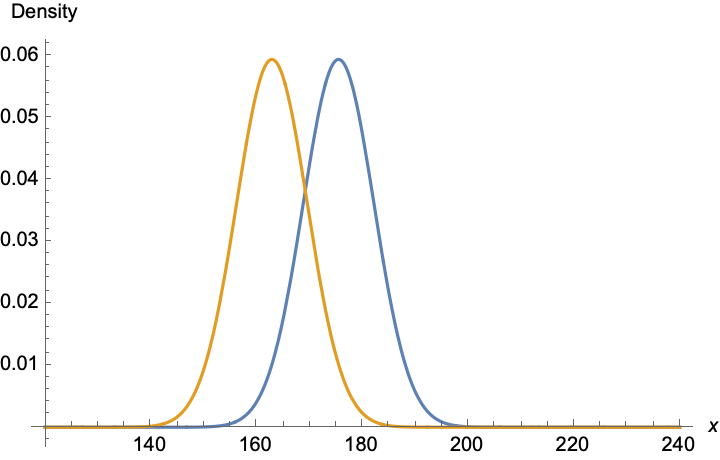
\includegraphics[width = 11cm]{bellCurves.png}
    \caption{Pdf of two normal distribution with common variance and different means}
    \label{bell}
\end{figure}
This model is, however, very simple and doesn't utilize the information from all other spectral bands. To do this, a multivariate model is constructed.

\subsection{Multivariate model}\label{sec:3_multivariate_model}
Every pixel in the multi-spectral images corresponds to meat or fat, as in the case above. Assuming that each pixel is an independent multivariate normal random variable, with distribution $\mathcal{N}(\boldsymbol{\mu}_i,\boldsymbol{\Sigma}),\:i\in\{1,2\}$, corresponding to meat or fat respectively. For a given pixel $\textbf{x}\in\mathbb{R}^n$ the mathematical problem is to determine whether $\textbf{x}\sim\mathcal{N}(\boldsymbol{\mu}_1,\boldsymbol{\Sigma})$ or $\textbf{x}\sim\mathcal{N}(\boldsymbol{\mu}_2,\boldsymbol{\Sigma})$.\\
When considering a single spectral band the 

An observation $\textbf{x}$ is most likely to be in class 1 if $P(C_1|\textbf{x})>P(C_2|\textbf{x})$ by Bayes formula i.e $P(\textbf{x}|C_1)P(C_1)>P(\textbf{x}|C_2)P(C_2)$. Due to the assumption of each class being multivariate normally distributed with prior probabilities $P(C_i)=p_i,\:i\in\{1,2\}$, these probabilities are known. By applying the logarithm and removing any terms not dependent on the class we define the threshold $S_i(\textbf{x})$ by,

\begin{align*}
    P(\textbf{x}|C_i)p_1&=\frac{1}{\sqrt{2\pi}^n\sqrt{|\boldsymbol{\Sigma}}|}\text{exp}\bigg[-\frac{1}{2}(\textbf{x}-\boldsymbol{\mu_1})^T\boldsymbol{\Sigma}^{-1}(\textbf{x}-\boldsymbol{\mu_i})\bigg]p_i \\
    S_i(\textbf{x})&=-\frac{1}{2}(\textbf{x}-\boldsymbol{\mu_i})^T\boldsymbol{\Sigma}^{-1}(\textbf{x}-\boldsymbol{\mu}_i)+\log(p_i) \\
    &=-\frac{1}{2}\big[\textbf{x}^T\boldsymbol{\Sigma}^{-1}-\boldsymbol{\mu}^T_i\boldsymbol{\Sigma}^{-1}(\textbf{x}-\boldsymbol{\mu}_i)]+\log(p_i)\\
    &=-\frac{1}{2}\big[\textbf{x}^T\boldsymbol{\Sigma}^{-1}\textbf{x}-\textbf{x}^T\boldsymbol{\Sigma}^{-1}\boldsymbol{\mu}_i-\boldsymbol{\mu}_i^T\boldsymbol{\Sigma}^{-1}\textbf{x}+\boldsymbol{\mu}_i^T\boldsymbol{\Sigma}^{-1}\boldsymbol{\mu}_i\big]+\log(p_i) \\
    &=\frac{1}{2}\big[\textbf{x}^T\boldsymbol{\Sigma}^{-1}\boldsymbol{\mu}_i+\boldsymbol{\mu}_i^T\boldsymbol{\Sigma}^{-1}\textbf{x}-\boldsymbol{\mu}_i^T\boldsymbol{\Sigma}^{-1}\boldsymbol{\mu}_i\big]+\log(p_i).
\end{align*}

Since $\boldsymbol{\Sigma}$, is symmetric we obtain  
\begin{align*}
    S_i(\textbf{x})&=\frac{1}{2}\big[\textbf{x}^T\boldsymbol{\Sigma}^{-1}\boldsymbol{\mu}_i+\boldsymbol{\mu}_i^T\boldsymbol{\Sigma}^{-1}\textbf{x}-\boldsymbol{\mu}_i^T\boldsymbol{\Sigma}^{-1}\boldsymbol{\mu}_i\big]+\log(p_i)\\
    &=\textbf{x}^T\boldsymbol{\Sigma}^{-1}\boldsymbol{\mu}_i-\frac{1}{2}\boldsymbol{\mu}_i^T\boldsymbol{\Sigma}^{-1}\boldsymbol{\mu}_i+\log(p_i).\\
\end{align*}

Using this threshold the classification for each pixel can be made from the following function.

\begin{align*}
    \tau(\textbf{x})=\begin{cases}
        C_1 \quad & S_1(\textbf{x})\geq S_2(\textbf{x}) \\
        C_2 \quad & S_2(\textbf{x})<S_1(\textbf{x}).
    \end{cases}
\end{align*}


\section{Results}
\subsection{Single spectral band}
Training errors \\
\begin{table}[H]
\begin{tabular}{|c|c|c|c|c|c|c|c|c|c|c|}
\hline
\textbf{Training day} & 1 & 2 & 3 & 4 & 5 & 6 & 7 & 8 & 9 & -\\
\hline
\textbf{Error} & 0.034 & 0.029 & 0.032 & 0.035 & 0.038 & 0.041 & 0.041 & 0.038 & 0.051 & -\\
\hline
\textbf{Training day} & 10 & 11 & 12 & 13 & 14 & 15 & 16 & 17 & 18 & 19 \\
\hline
\textbf{Error} & 0.047 & 0.057 & 0.054 & 0.053 & 0.067 & 0.064 & 0.061 & 0.057 & 0.059 & 0.115 \\
\hline
\end{tabular}
\caption{Training errors for all uni variate models}
\label{tab:univariate-errors}
\end{table}
%\\Test error for 2nd spectral band2\\
\begin{table}[H]
\begin{tabular}{|c|c|c|c|c|c|c}
\hline
Test day & 01 & 06 & 13 & 20 & 28 \\
\hline 
Training day: 06 & 0.035 & - & 0.066 &0.074 & 0.065 \\
\hline
\end{tabular}
\caption{Test errors for the best single spectral band.}
\label{tab:univariate-errors-day6}
\end{table}
\subsection{Multivariate model}
Based on the multivariate model described in Section \ref{sec:3_multivariate_model} we first start by assuming that the prior probability for fat is $p_1 = 0.5$ and get the following table.

\begin{table}[H]
    \centering
    \begin{tabular}{|c|c|c|c|c|c|c}
        \hline
        Test day & 01 & 06 & 13 & 20 & 28 \\
        \hline
        Training day: 01 & - & 0.068 & 0.053 & 0.099 & 0.146 \\
        Training day: 06 & 0.025 & - & 0.021 & 0.034 & 0.033 \\
        Training day: 13 & 0.042 & 0.059 & - & 0.051 & 0.064 \\
        Training day: 20 & 0.035 & 0.055 & 0.035 & - & 0.039 \\
        Training day: 28 & 0.040 & 0.062 & 0.036 & 0.049 & - \\
        \hline
    \end{tabular}
    \caption{Error rate with prior probability for fat $p_1 = 0.5$}
    \label{tab:multivariate-simple-prior}
\end{table}

From Table \ref{tab:multivariate-simple-prior} we see that by training on day 6 the overall error rate for the remaining days are all lower than their corresponding counterparts. 

If we instead use the fact that there is $30\%$ fat in the sense that the prior probability for fat becomes $p_1 = 0.3$ we get the following table.

\begin{table}[H]
    \centering
    \begin{tabular}{|c|c|c|c|c|c|c}
    \hline
    Test day & 01 & 06 & 13 & 20 & 28 \\
    \hline
    Training day: 01 & - & 0.058 & 0.041 & 0.081 & 0.123 \\
    Training day: 06 & 0.021 & - & 0.017 & 0.027 & 0.027 \\
    Training day: 13 & 0.038 & 0.053 & - & 0.044 & 0.054 \\
    Training day: 20 & 0.030 & 0.048 & 0.028 & - & 0.031 \\
    Training day: 28 & 0.035 & 0.054 & 0.029 & 0.041 & - \\
    \hline
    \end{tabular}
    \caption{Error rate with prior probability for fat $p_1 = 0.3$}
    \label{tab:multivariate-correct-prior}
\end{table}

From Table \ref{tab:multivariate-correct-prior} we see that by training on day 6 the overall error rate for the remaining days are all lower than their corresponding counterparts. 
We also note that by comparing Table \ref{tab:multivariate-correct-prior} with Table \ref{tab:multivariate-simple-prior} that the overall error rate is lower. 


\begin{figure}[H]
    \centering
    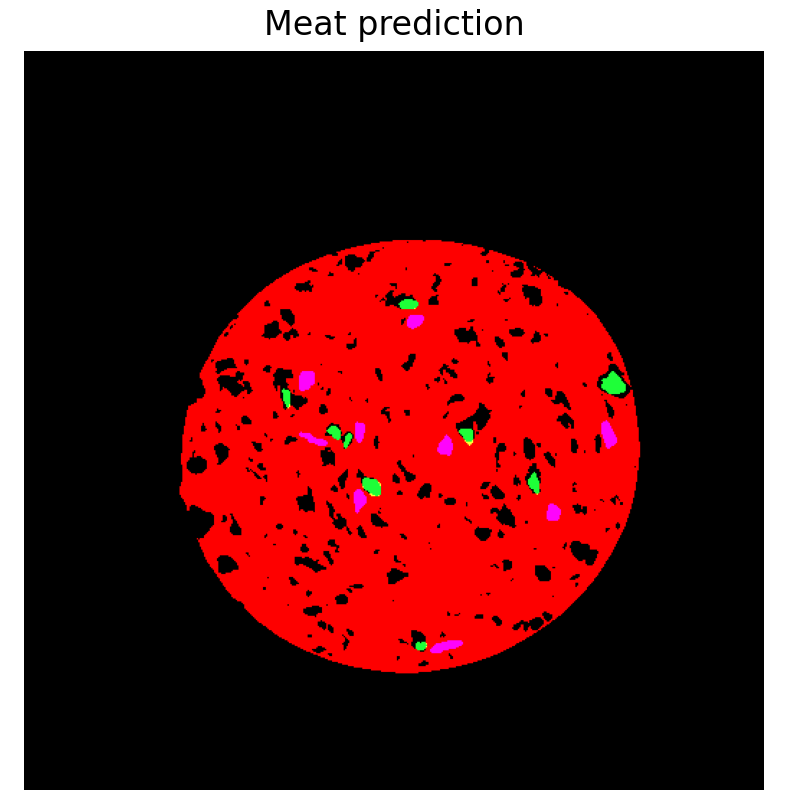
\includegraphics[width = 7cm]{meatPrediction.png}
    \caption{Illustration of predicted fat (black), predicted meat (red), annotated fat (green) and annotated meat (pink).}
    \label{meatpredict}
\end{figure}

\section{Validity of the model}
 

\section{Conclude}
As illustrated in tables \ref{tab:univariate-errors} and \ref{tab:univariate-errors-day6}, even a simple univariate model based on the best spectral band on a single image, see section \ref{sec:3_univariate_model}, can predict the position of fat and meat in other images reasonably well. \\
But by utilizing information from all spectral bands, we can, as might be expected, get a much more accurate model - see figure \ref{meatpredict} and table \ref{tab:multivariate-correct-prior}. \\
A complete python implementation is provided in the appendix, which allows for easy reproducability of our results. Moreover, a github repository with additional functionality and analysis is provided here \url{https://github.com/ElMiho/02525-project-2}.



\section{References}
\begin{thebibliography}{9}
\bibitem{Videometer}
Videometer, \emph{videometer.com/videometerlab/}, visited: 12/03-23
\end{thebibliography}

\newpage
\appendix
\section{Code}
All of the following code can also be seen on \url{https://github.com/ElMiho/02525-project-2}
\subsection{Code for single spectral band}
\lstinputlisting[language=Python,breaklines=true]{code/single_spectral_band.py}

\subsection{Code for all spectral bands}
\lstinputlisting[language=Python,breaklines=true]{code/all_spectral_bands.py}

\subsection{Calculation for all days}
\lstinputlisting[language=Python,breaklines=true]{code/calculation_all_days.py}

\subsection{Generation of tables}
\lstinputlisting[language=Python,breaklines=true]{code/Error_Multivariate.py}



\end{document}